\chapter{Testing with a timing component}\label{sec:topic_4}

% Tobias_Koch

\section{Introduction}

Requirements are the basis for all testing. In practice, requirements
are often available in a wide variety of formats: As natural language
text, spreadsheets, UML diagrams etc.... In addition to that, requirements
are often not close to testing. In the course of the development phases
of a program, the requirements may expand or change. In industry,
individual software components are often developed by different manufacturers
before they are combined into a system by the client of these productions.
Although components are tested individually and independently, many
errors can only be discovered when the components are integrated.
Therefore Test cases and requirements must be more closely linked.
Flaws and vagueness in requirements are common and hard to discover.
\enquote{On account of this testing time may be wasted with test
cases that result in the detection of flaws in the requirements and
can thus not be used to evaluate the system under test (SUT)}
\cite{Siegl2010}. Therefore requirements must be stricter and more
formal.\\
 Furthermore, there are systems that have to fulfil real-time requirements.
Two approaches (Chapter \ref{sec:Approach-1} and \ref{sec:Approach-2})
will be presented in this chapter. Both approaches test with a time
component as they refer to a real-time system. In these systems, it
is not only important what input the individual system functions receive
(for example, through a boundary value analysis), but also how long
they take. The same input in a real-time system can lead to a different
system reaction if the execution time differs. But not only the execution
duration of a system function, also the time between the execution
of a system function can result in another system reaction. For this
reason, the temporal aspect plays a major role in the approaches.\\
 \\
The first approach with the title \enquote{Model Based Requirements
Analysis and Testing with Timed Usage Models (TUM)} is a graphically
representation of requirements specification. \enquote{During
the creation of the model the requirements are analysed and brought
into an unambiguous and formal representation} \cite{Siegl2010}.
Test cases are automatically generated from the graph using EXAM (Extended
Automation Method). The second approach, \enquote{A Model-Based
Testing Technique for Component-Based Real-Time Embedded Systems}
(in addition to the formal specification of the requirements by models),
deals even more specifically with the dependency between individual
components of SUT, so that they are taken into account in the automatic
test generation from these models.\\
 \\
Chapter \ref{sec:Literature-Search} explains the process of the literature
search that was used to find the second approach. Chapter \ref{sec:Comparison}
compares the two approaches and shows the result in a synthesis matrix.
Chapter \ref{sec:topic_4_Conclusion} provides an assessment of the approaches
and summarises the most important findings.\\
Please refer to the glossary in order to receive a common understanding of the following terms used in the sections below: SUT, CACC, TUM, EXAM, CREMTEG, CIIG, CSIBG, CSIEDBG, AIC, AITC, AIEC.

\section{Literature Search\label{sec:Literature-Search}}

The literature search was conducted in too ways: Search term and snowballing.
To find more and possibly different approaches the search question
was chosen to be: \enquote{What models with a timing component
exist that favor the creation of automatically generated tests?}
The ACM \cite*{acm} and IEEE \cite*{ieee} search sources were considered.
Relevance criteria, both substantive and formal, were used to limit
the number of search hits. 
\begin{itemize}
\item Content criteria: \enquote{requirements as a core concept},
\enquote{support for automatically generated tests},
\enquote{model with consideration of timing}. 
\end{itemize}
The content criteria were first searched for throughout the document.
Since the number of hits was too large, the search of the content
criteria was limited to the abstract of the article. 
\begin{itemize}
\item Formal criteria: time criterion, diversity of author and language
of article in English. 
\end{itemize}
The time criterion was initially chosen so that only articles that
were not older than ten years (publication date not less than 2010)
were considered. Since the number of hits was still too large, the
time criterion was finally set to 2015. The difference of the author
from the given article should ensure that a second independent, not
subjectively biased, scientific opinion on the topic \enquote{Testing
with a time component} could be found.\\
Forward Snowballing produced 13 results, two of which were relevant
(according to the criteria). Backward Snowballing also produced 13
results, none of which were relevant. All of the results did not meet
the time criterion, as the given article was from 2010. Table 1.1
shows an overview of the search-term-based literature search.\\
 
\begin{table}[h]
	\centering
	\caption{Overview of the search-term-based literature search}
	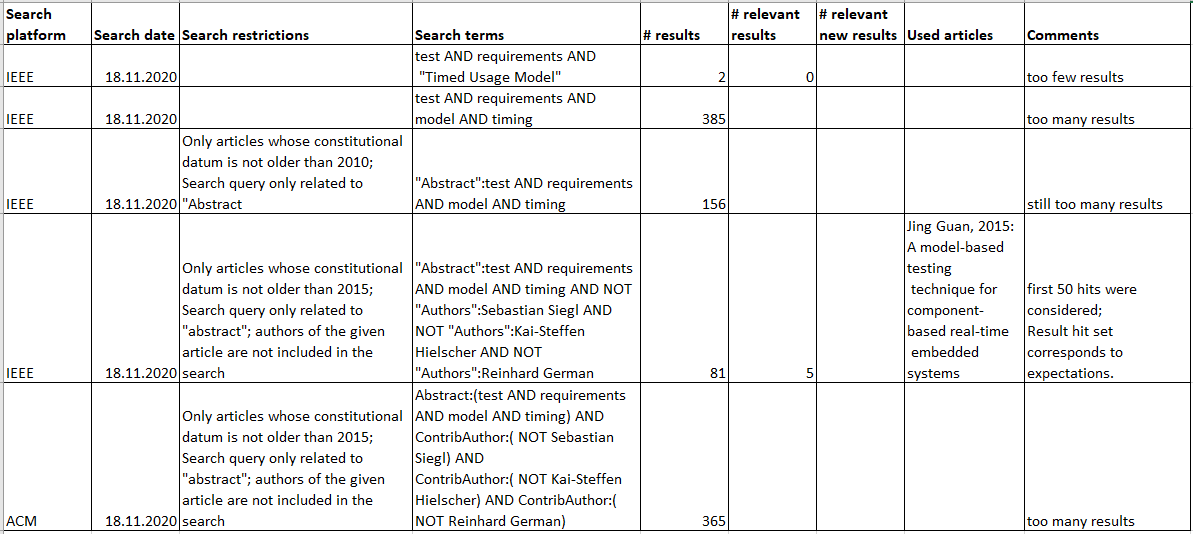
\includegraphics[scale=0.8]{../images/SearchTermTable} 
\end{table}
The search term in the first literature search method used was initially
too specific (test AND requirements AND \enquote{Timed Usage
Model}). This was generalised in the next step to increase
the number of hits in the search query: \enquote{test AND requirements
AND model AND timing}. This type of search was able to
optimally fulfill the content criteria and the formal criteria. In
combination with the previously mentioned criteria and the further
restriction of the search that the search term only refers to the
abstract of the article, the literature on which approach 2 is based
was selected.

\section{Approach 1: Model Based Requirements Analysis and Testing with Timed
Usage Models\label{sec:Approach-1}}

\subsection{Description}

In practice, requirements often exist in a wide variety of formats.
A stricter formal notation of the requirements can be achieved through
the so-called TUM (Timed Usage Model). During the creation of the
model, the requirements are analysed and brought into a uniform form.
Each path in the model is ultimately based on a requirement: in this
way, the relationship between the previously created requirements
and the later model-based requirements can be traced at any time.
Each requirement must be simultaneously retrievable in a \enquote{path}
of the TUM. The expected system reaction, after a requirement has
been executed, must be marked in the diagram by means of an (end-)
state. \enquote{Design} errors can be detected early
in the creation of the model. The special feature of the model is
the consideration of the time aspect: The states and state transitions
in the model are each assigned a probability density function (pdf),
which calculates the time how long the system remains in a certain
state or how long the execution of an operation or a response of the
SUT takes. Each state transition is therefore assigned a stimulus,
which represents an operation of the SUT or a system response. Figure
1.1 shows an easy example for a TUM: \enquote{S}
are states, \enquote{a} stands for state transition,
\enquote{t} describes a pdf either with respect
to a state or to a transition, and \enquote{p} describes
the transition probability from one state to the next.

\begin{figure}[H]
	\centering
	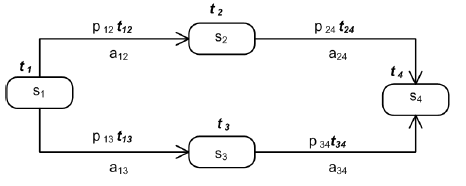
\includegraphics{../images/TUM}
	\caption{TUM \cite{Siegl2010}}
\end{figure}
The model serves as the basis for the entire testing process. It is
used in the testing of real-time systems, e.g. in the automotive industry
or in energy management. The model is created manually using a specially
developed editor. \\
It is done in two steps: First, the system boundary will be defined.
Second, all sequences of stimuli and their responses across the system
boundary will be enumerated \cite{Siegl2010}. All stimuli that go
across this boundary are extracted from the existing requirements
\cite{Siegl2010}. Each possible sequence of stimuli will be mapped
to a response of the system. A response can be composed of one or
more outputs. \enquote{Two sequences u and v are equivalent if
extended by any sequence w the future response is the same to uw and
vw} \cite{Siegl2010}. These equivalent sequences are
reduced to one sequence, since testing the other sequences would be
redundant. In order to maintain an overview of the large number of
all possible sequences, they are listed in order of length: It starts
with an empty sequence \textlambda{}
and all sequences of length one
are created first, then all sequences of length two and so on. By
this procedure a complete and consistent usage model is created. The
finished TUM is passed to EXAM in the next step. \enquote{EXAM
comprises the automated generation of platform dependent code and
the automated execution of the derived test suite without human interactions}
\cite{Siegl2010}. Test cases are automatically generated by running
through the different paths of the TUM. All paths from the start to
the final state are valid test cases.\\
For the test oracle, an appropriate counterpart from the EXAM test
automation library is assigned to each individual stimulus. An importer
allows thereby the import of a requirements library from a document-based
requirements management system. The elements of this system can be
traced back to each individual object in the TUM. The reference values
or the expected result of one \enquote{test path}
for the test oracle can be derived in three different ways: First
automatically generated by computation rules, second by a textual
description (program code or natural language) and third by measurements
and checks on test benches.

\subsection{Application}

The approach \enquote{Model Based Requirements Analysis and Testing
with Timed Usage Models} will now be applied to the Movie Manager,
a collaborative project of students. The program comes with a domain
diagram, an overview of all system functions, and a user task sheet
about movie management in natural language. This data was used in
the creation of the TUM. Data on the transition probability from one
state to the next state is not available. This is therefore considered
to be identical for all state transitions. In order to nevertheless
realise a temporal component in the Movie Manager, the requirements
were extended in the following way: Within the subtasks \enquote{Describe
a movie} and \enquote{Describe a performer},
changes were made to the system functions \enquote{show movie
in IMDB} and \enquote{show performer in IMDB}:
After the error message \enquote{Connection failed}
appears, the system should automatically try to establish a connection
to the IMDB website \cite*{imdb}. If this exceeds a certain time
value (in this case 120 sec.), a final message is issued to the user
stating that the connection could not be re-established automatically.
After this message appears, no further attempts are made to connect
automatically to the IMDB server.

\begin{figure}[H]
	\centering
	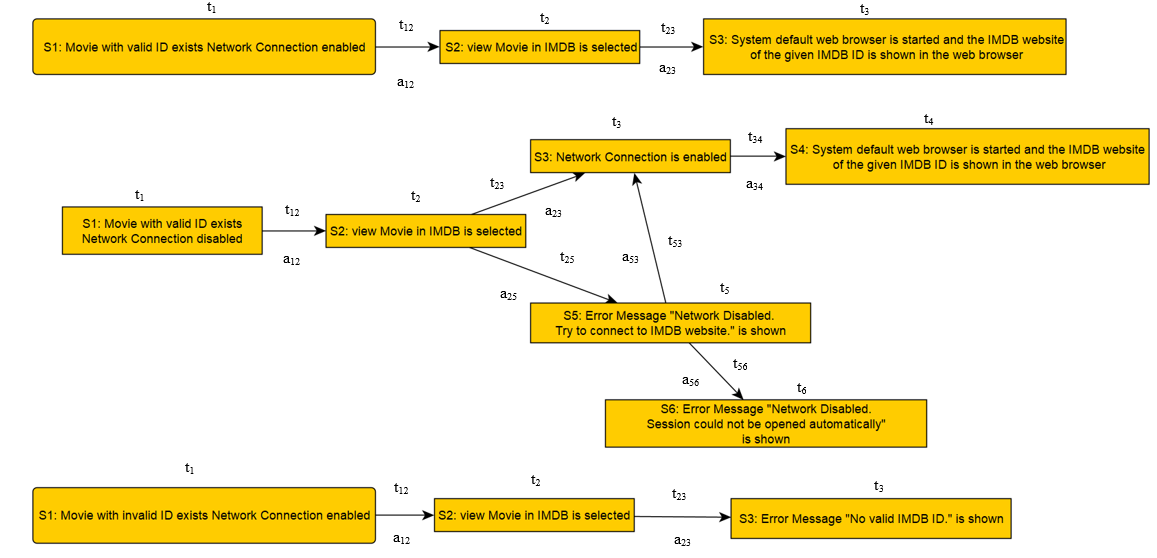
\includegraphics[scale=0.8]{../images/Application1_MovieManager} 
	\caption{TUM for the systemfunction \enquote{view Movie in IMDB} in Movie Manager}
\end{figure}
The middle graph in Figure 1.2 shows the time dependency: As soon
as t5 \textgreater{} 120 (unit in sec.), the state changes from
S5 to S6. If the network connection has been re-established before
120 sec. have elapsed, the system switches to state S3. The graph
includes all sequences that are conceivable when calling the system
function \enquote{view Movie in IMDB}. In the next
step, a test suite could be automatically created from the graph using
EXAM by traversing all paths in the graph. The exact procedure of
this step is not described in detail in the approach.

\section{Approach 2: A Model-Based Testing Technique for Component-Based Real-Time
Embedded Systems\label{sec:Approach-2}}

\subsection{Description}

Component-based modeling of embedded systems is becoming more and
more important in the field of \enquote{software engineering}
due to the increasing complexity of the systems. The approach now
shows possibilities to improve the quality of tests of component-based
embedded systems by means of several graph-based test models. The
focus is particularly on non-functional requirements, more precisely,
real-time requirements. The appropriate testing of these is often
neglected during the integration of the individual components in a
real-time embedded system. The test models presented here (except
for the CIIG (Component Interface Interaction Graph), which only fulfills
the former) take into account not only the functional and temporal
dependencies between individual components, but also the temporal
dependency between state transitions within a component. All the models
presented are created manually using a tool. In the following, it
will be briefly explained how and from which data the models are collected,
which elements they consist of and in which respects they differ.

\begin{figure}[H]
\centering{}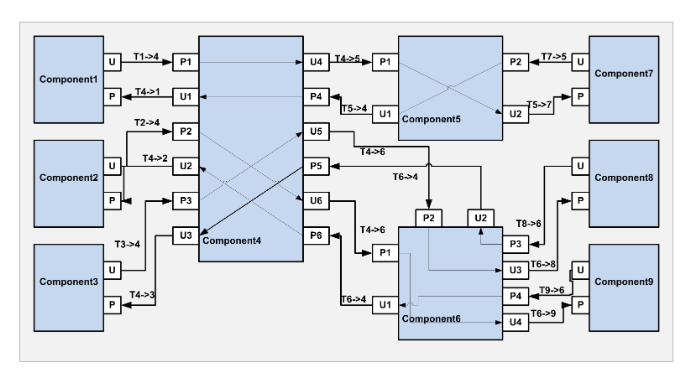
\includegraphics{../images/CIIG}\caption{CIIG \cite{Guan2015}}
\end{figure}
The CIIG, shown in Figure 1.3, can be derived from architecture framework
and design specifications, that specify the primary components, interfaces
and dependencies of softwaresystems, for example by context diagrams
or sequence diagrams \cite{Guan2015}. For the CIIG, a component subnet
is created for each component in the sequence diagram. Also, the external
and internal message edges and provider/user interfaces can be derived
from component level sequence diagrams. For each message in the sequence
diagram, a component provider interface, a component user interface
and an external message edge is created. Additionally, one internal
component message edge is created between two external message edges.\\
The CIIG consists of a set of components, which in turn have a certain
number of user (U) and provider interfaces (P). The paths in the model
are defined via so-called message-edges. Internal message edges determine
from which provider interface to which user interface the message
can be sent in a component. External message edges determine from
which user interface to which provider interface the message can be
sent between individual components. Each external message edge is
assigned to a time stamp (for example T1-\textgreater 4), which stores
the transmission time of the message. \\
\enquote{A CIIG represents the time-dependent connectivity relationships
between these components as well as time-dependent relationships inside
a component {[}...{]}. But a CIIG does not reflect the internal behaviour
of a component {[}...{]}} \cite{Guan2015}. This is realized
by a CSIBG (Component State-based Interaction Behavior Graph), shown
in Figure 1.4.

\begin{figure}[H]
	\centering
	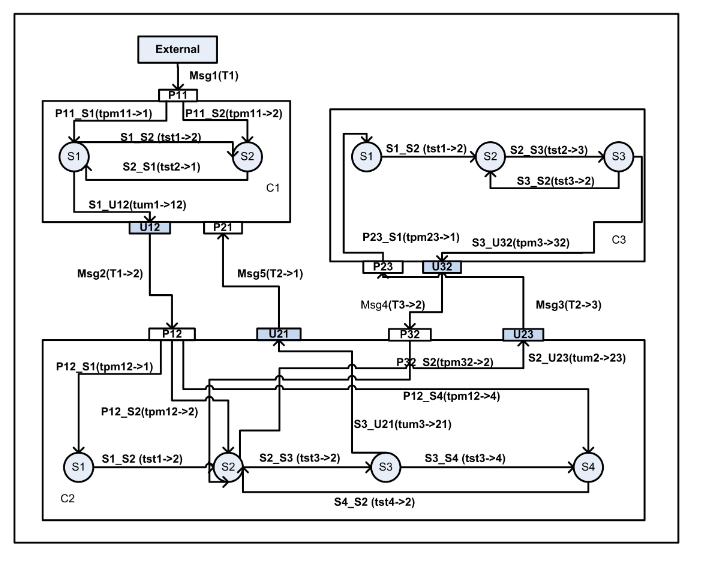
\includegraphics{../images/CSIBG} 
	\caption{CSIBG \cite{Guan2015}}
\end{figure}
\enquote{A CSIBG is created from a CIIG and state transitions
in state diagrams for each corresponding component. Test paths are
generated from the CREMTEG CSIBG diagram {[}...{]}} \cite{Guan2015},
since in this diagram the maximum number of possible paths that can
occur through method calls or state transitions has been created:
The number of test paths is equal to the product of the number of
all possible transition paths in each individual CSIBG component subnet.
In this model, in addition to the CIIG, all internal states (S) ,
state transitions (for example S1\_S2), transitions between Provider
Interfaces and internal states (for example P12\_S1), transitions
between states and User Interfaces (for example S2\_U23) and time
dependencies between individual states (for example tst1-\textgreater
2) and between the states and the provider (for example tpm12-\textgreater
1) or user interfaces (for example tum2-\textgreater 23) of a component
are represented. The most comprehensive model is the CSIEDBG (Component
State-based Event-driven Interaction Behavior Graph).

\begin{figure}[H]
	\centering
	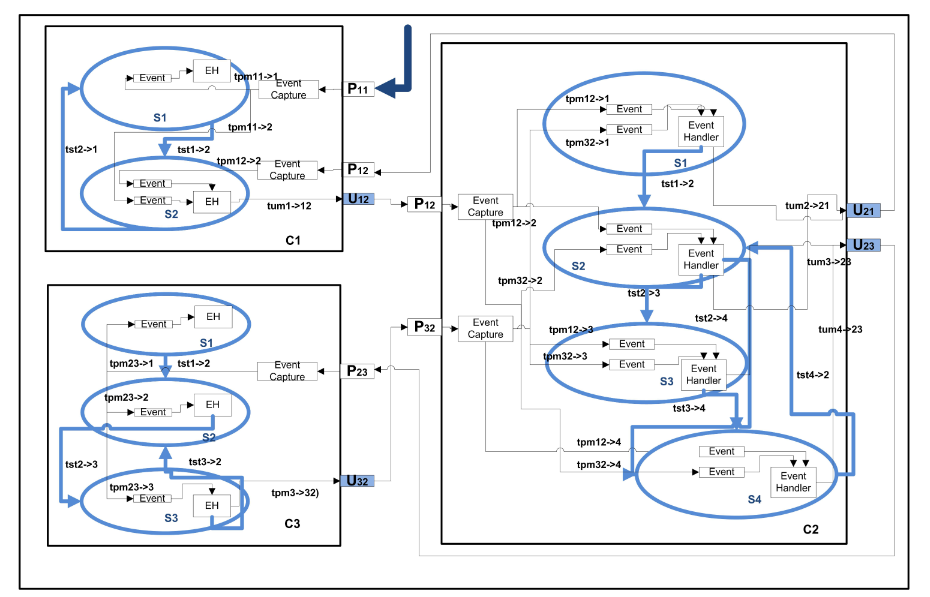
\includegraphics{../images/CSIEDBG} 
	\caption{CSIEDBG \cite{Guan2015} }
\end{figure}
\enquote{CIIG and CSIBG clearly described the time sequences
of method calls and paths of state transitions, but they do not deal
with concurrency} \cite{Guan2015}. The CSIEDBG additionally
considers multitasking and non-deterministic behavior, e.g., when
processing simultaneously generated messages. Therefore, the model
in Figure 1.5 is extended as follows: Each provider service in a component
has one event capture. Each state in a component contains one event
handler (EH) \cite{Guan2015}. \enquote{The provider component
processes the message by event capture to generate events in the current
component state. All generated events are sent to event handler to
decide whether to transition to the next state or send an outgoing
message to the next component {[}...{]}. Decisions in the event handler
are modeled as predicate expressions, where each clause is an event.}
\cite{Guan2015}. New test paths are created according to CACC (Correlated
Active Clause Coverage). CACC is a special form of predicate logic.
For the exact definition of CACC, see the glossary.\\
The models are used to automatically generate test specifications
for component integration testing \cite{Guan2015}. The procedure
is not described in more detail in the approach. The implementation
of the test cases from the test specification is not automated. To
evaluate the suitability of the models, the test suites are run under
a system in which manual errors have been introduced \cite{Guan2015}.
Test Data were hand generated. \enquote{Test data were taken
as inputs to a proprietary test automation tool {[}...{]} . The test
tool reads the input test procedure files, launches the software,
waits for the test to complete, retrieves output log files and analyzes
the results to determine whether test was successful {[}...{]}. A
final test report was generated after all tests were run}
\cite{Guan2015}.\\
The results of the approach have shown that the function and block
coverage and fault detection rate could be significantly improved
by using a CSIEDBG compared to a CIIG or CSIBG. However, in a complex
real-time embedded system, it is often impossible to cover all test
paths. For this reason, it must be decided on a case-by-case basis
which test approach is chosen. Each model fulfills a test criterion
of different quality: A CIIG fulfills the All-Interface Coverage Criterion
(AIC). ``This criterion ensures that each interface is tested once''
\cite{Guan2015}. A CSIBG fulfills the All-Interface-Transition Coverage
Criterion (AITC). ``This criterion ensures that each interface between
components is tested once and each internal state transition path
in a component is toured at least once'' \cite{Guan2015}. A CSIEDBG
fulfills the All-Interface-Event Coverage Criterion (AIEC). ``AIEC
combines edge coverage with logical coverage'' (see above) \cite{Guan2015}.
Models presented here serve as a basis for the creation of automatically
generated test cases.

\subsection{Application}

The interaction between individual components is now applied to the
Movie Manager Application, shown in Figure 1.6. In order to maintain
clarity, the labels above the message edges are omitted as far as
possible. The various widgets within the Movie Manager form the components
in the overall system. Within these components there are states (e.g.
under the component \enquote{Movies Tab} there is
a state \enquote{empty} if no movies are stored
in the movie list and a state \enquote{Movies List}
if at least one movie is stored). The message edges show the information
exchange of the existing system functions. Multi threading does not
play a role in the Movie Manager, so a CSIBG was used for the demonstration.

\begin{figure}[H]
\centering{}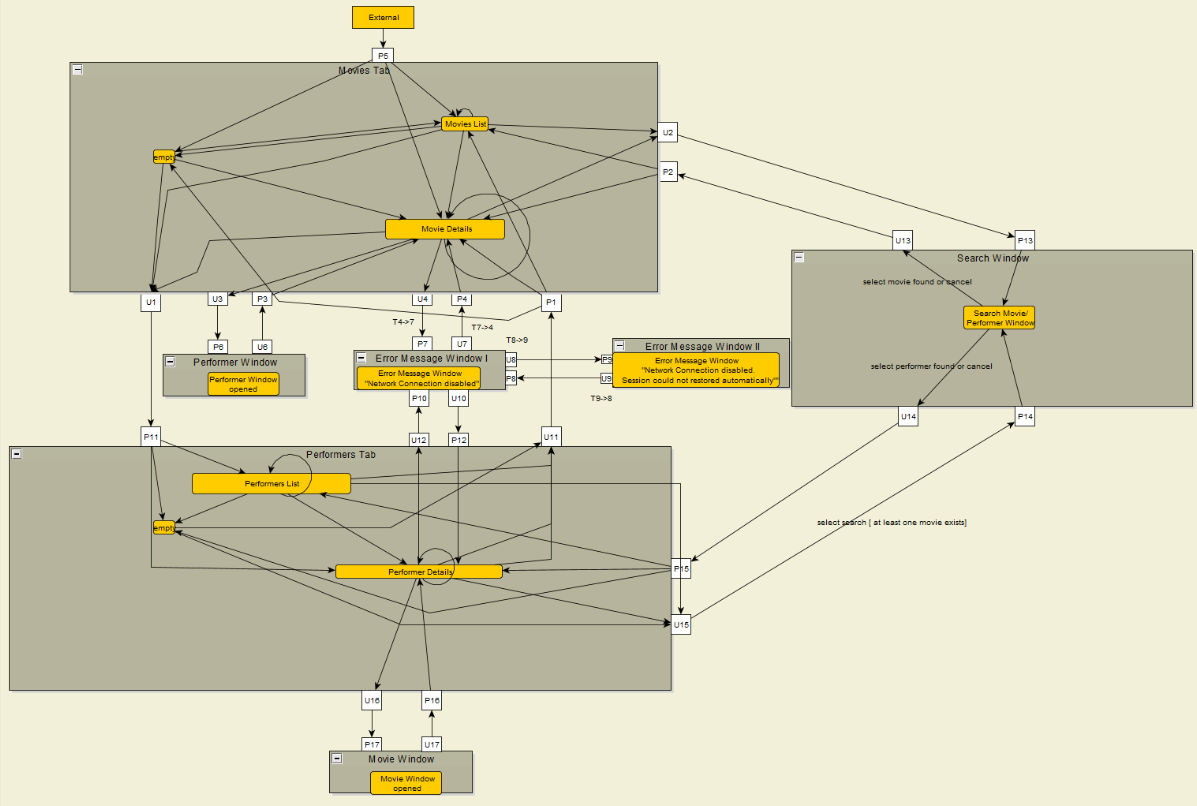
\includegraphics[scale=0.8]{../images/Application2_MovieManager}\caption{CSIBG for the Movie Manager application}
\end{figure}
Legend for graph shown in Figure 1.6: The grey rectangular boxes are
components of the movie manager, the yellow boxes are the states in
a component, the small rectangular boxes on the edge of a component
are User- (U) or Providerinterfaces (P). Arrows symbolize intern (in
a component) and extern (between components) messages. \enquote{T}
are time stamps at external component messages. \\
The system functions \enquote{show Movie in IMDB}
and \enquote{show Performer in IMDB}, which have
already been modified in approach 1, are extended by the following
function: The error message window \enquote{Network Connection
disabled} is to be closed automatically if the network
connection could be restored before 120 seconds have elapsed. For
this example (T7-\textgreater 4) - (T4-\textgreater 7) must be smaller
or equal 120. The Message Edge between U8 and P9 only exists, if (T8-\textgreater
9) - (T4-\textgreater 7) is greater than 120.

\section{Comparison\label{sec:Comparison}}

\begin{longtable}[l]{|>{\centering}p{2cm}|>{\centering}p{2.5cm}|>{\centering}p{5cm}|>{\centering}p{5cm}|}
\hline 
Number  & Name  & Approach 1(\ref{sec:Approach-1})  & Approach 2(\ref{sec:Approach-2})\tabularnewline
\hline 
\hline 
3a)  & Which artifacts and relations between artifacts are used in the approach?
Which artefacts are created in the course of the approach? How are
the artifacts characterized?  & Requirements specification: This could be natural language text, spreadsheets,
drawings or UML charts. TUM: Will be manually derived from the requirements
specification by a special tool. Test Cases: These are automatically
derived from a TUM and executed by EXAM.  & CREMTEGs were manually created with a tool from software architecture
and design specifications (like Graphs, sequence diagrams, state diagrams,
grammars, logical expresses and input domains). The CIIG can be derived
from architecture framework and design specifications, that specify
the primary components, interfaces and dependences of software systems,
for example by context diagrams or sequence diagrams. A CSIBG is created
from a CIIG and state transitions in state diagrams for each corresponding
component. A CSIEDBG is an extended version of the CSIBG. It includes
handling with events for multitasking. Test specifications were automatically
developed from CREMTEGs. An test tool reads the input test procedure
files, launches the software, and waits for the test to complete.\tabularnewline
\hline 
3b)  & What is required and/or input for the application of the approach?  & Requirements specification in different formats. System boundary is
clearly defined.  & System boundary must (particularly because the approach stays in relation
with an embedded system) clearly be defined. Software architecture
and design specification, from which the data for the models are derived.\tabularnewline
\hline 
3c)  & What steps does the approach consist of? Which information is used
in which step and how?  & The TUM model is created in two steps: First, the system boundary
will be defined. Second, all sequences of stimuli and their responses
across the system boundary will be enumerated. All stimuli that go
across this boundary are extracted from the existing requirements.
Each possible sequence of stimuli will be mapped to a response of
the system. The sequences are created in ascending order of length.
By this procedure a complete and consistent usage model is created.
The finished TUM is passed to EXAM in the next step. After the import,
test cases are automatically generated by running through the different
paths of the TUM. For the test oracle, an appropriate counterpart
from the EXAM test automation library is assigned to each individual
stimulus. An importer allows thereby the import of a requirements
library from a document-based requirements management system. The
elements of this system can be traced back to each individual object
in the TUM.  & First the CREMTEGs will be constructed. For the CIIG, a component
subnet is created for each component in the sequence diagram. A CSIBG
is created from a CIIG and state transitions in state diagrams for
each corresponding component.Test specifications for the test cases
are automatically created from the finished CREMTEGs. The implementation
of the test cases from the test specification is not automated. Finally,
the test cases created from the CREMTEGs are run through in the SUT.
Test Data were hand generated. \enquote{Test data were taken
as inputs to a proprietary test automation tool {[}...{]} . The test
tool reads the input test procedure files, launches the software,
waits for the test to complete, retrieves output log files and analyzes
the results to determine whether test was successful {[}...{]}. A
final test report was generated after all tests were run}\cite{Guan2015}. \tabularnewline
\hline 
4a)  & Which usage scenarios are supported by the approach?  & Automatically generated test cases are created from the requirements;
testing possible at both system and component level. Test time reduced
(through early error detection in requirements and the related incorrect
creation of test cases). Avoidance of ambiguities in the description
of requirements to prevent errors in test creation. Acceptance criteria
such as test coverage can be achieved more easily with the help of
the model. Requirements are less likely to be misunderstood during
software development for the reasons mentioned.  & The basis for the usage scenario is a component-based embedded real-time
system. The test technique is used to put the internal processes (such
as state transitions, event handling) in relation to the required
time and thus create a more transparent test model, which improves
the error detection rate in the system and the general code coverage
of the system.\tabularnewline
\hline 
4b)  & Which stakeholders are supported by the approach?  & Test designer in the software team, Software developer, Requirements
Engineer  & Test design team (must be familiar with software architecture design
e. g. to analyze UML diagrams, needs advanced domain knowledge)\tabularnewline
\hline 
4c)  & Which knowledge areas from SWEBOK can be assigned to the usage scenarios?  & Software Requirements \textrightarrow{} Requirements Analysis \textrightarrow{}
Formal Analysis,

Software Requirements \textrightarrow{} Requirements Validation \textrightarrow{}
Model Validation,

Software Testing \textrightarrow{} Test Levels \textrightarrow{} The
Target of Tests,

Software Testing \textrightarrow{} Test Levels \textrightarrow{} Objectives
of Testing,

Software Testing \textrightarrow{} Test Techniques \textrightarrow{}
Model-Based Techniques,

Software Engineering \textrightarrow{} Models and Methods \textrightarrow{}
Analysis of Models \textrightarrow{} Analyzing for completeness,

Software Engineering \textrightarrow{} Models and Methods \textrightarrow{}
Analysis of Models \textrightarrow{} Analyzing for consistency,

Software Engineering \textrightarrow{} Models and Methods \textrightarrow{}
Analysis of Models \textrightarrow{} Analyzing for correctness,

Software Engineering \textrightarrow{} Models and Methods \textrightarrow{}
Analysis of Models \textrightarrow{} Traceability  & Software Requirements \textrightarrow{} Requirements Analysis \textrightarrow{}
Formal Analysis,

Software Requirements \textrightarrow{} Requirements Validation \textrightarrow{}
Model Validation,

Software Requirements \textrightarrow{} Requirements Validation \textrightarrow{}
Acceptance Tests,

Software Testing \textrightarrow{} Test Levels \textrightarrow{} The
Target of Tests,

Software Testing \textrightarrow{} Test Levels \textrightarrow{} Objectives
of Testing,

Software Testing \textrightarrow{} Test Techniques \textrightarrow{}
Model-Based Techniques \tabularnewline
\hline 
5a)  & Which tool support is provided for the approach?  & An editor for the creation of Timed Usage Models, Requirement Management
System, EXAM, appropriate counterpart from the EXAM test automation
library  & Editor for creating the CREMTEGs, Program for generating automatically
test specifications from CREMTEGs, tool which starts the test and
determines whether test was successful\tabularnewline
\hline 
5b)  & Which steps of the approach are automated by a tool? Which steps are
supported by a tool, but still have to be executed manually? Which
steps are not supported by a tool?  & The creation of the TUMs is achieved using an editor, but must be
generated manually. EXAM includes the automatic generation of platform
dependent code and the automatic execution of the raised test suite
completely without human interaction.  & The CREMTEGs are created manually using an editor. The creation of
the test specification from the CREMTEGs is automated. The implementation
of the test cases from the test specification is not automated. Test
value generation and fault insertion must be done by hand. A tool
starts the test and determines whether test was successful automatically.\tabularnewline
\hline 
6a)  & How was the approach evaluated?  & The approach was evaluated in the testing of a \enquote{start-stop
functionality} (power train functionality) and energy
management in a car. The degree of coverage of the requirements in
manually created test cases was compared with the resulting degree
of coverage in the automatically generated creation of test cases
based on TUM. The advantages of a TUM were already evaluated during
its creation from the requirements.  & The approach was evaluated on an existing component-based embedded
system (satellite communication system written in C and C++, 75000
lines of code). The system was defined using sequence and state diagrams.
The system was then modified by mutation-based fault implementation
to verify the suitability of the design-based test models.\tabularnewline
\hline 
6b)  & What are the (main) results of the evaluation?  & The automatic creation of test cases covers a wider range of operation
sequences. The coverage of requirements was systematically increased.
System responses caused by the given functionality were partially
undefined (discovered during the creation of TUM). Requirements were
cleansed of deficits, shortcomings, contradictions and ambiguities.  & The use of extended design-based models in the generation of test
cases achieves a better error detection rate and a higher code coverage
(both function and block coverage) than the manual collection of test
cases. The interaction of internal states of the system (i.e. in the
individual components) could be made more transparent.\tabularnewline
\hline 
\end{longtable}Both approaches are presented to automate tests while taking a temporal
component into account. Approach 1 places particular emphasis on analysing
and \enquote{cleaning up} the existing requirements
of ambiguities, deficits and shortcomings. The procedure in this approach
is partly manual, partly automated: TUMs are created from the existing
requirements using an editor. Design errors of the requirements can
be detected during the creation of the model. EXAM allows the automatic
import of the TUM. EXAM generates code for the implementation of the
test cases and executes the test suite automatically. The level of
automation of the approach is therefore very high. In the second approach,
Component-Based Real Time Embedded Model-Based Test Graphs are generated
manually from the existing architecture and design specification.
Similar to the first approach, requirements are unified and thus freed
from ambiguities. Real-time requirements, i.e. requirements that are
linked to a time condition, are the main focus of testing. The level
of detail of a CREMTEG CSIBG or CSIEDBG is significantly higher than
that of a TUM. The special feature of the approach is that for the
first time information from component level sequence diagrams and
statecharts are combined to derive a graph based test model with timing
properties for test generation. From the CREMTEGs, a test specification
for component integration testing can be automatically generated.
The test suite must still be created manually from the test specification.
Test data and seeding of faults in the system are also created manually.
The second approach therefore has a low level of automation. The use
of advanced design-based models (supporting AITC and AIEC) in the
generation of test cases achieves a better fault detection rate and
a higher code coverage (both function and block coverage) than the
method used AIC.

\section{Conclusion\label{sec:topic_4_Conclusion}}

The literature search has shown that the topic of \enquote{testing
with a timing component} is not yet particularly widespread
in the industry. The search query \enquote{test AND requirements
AND Timed Usage Model} yielded only two
search hits, whereby both articles found were by the same author.
The second approach describes that it is very difficult to get access
to running real-time embedded systems, which are necessary to evaluate
the approach. Some intermediate steps have to be done by hand. Therefore,
this approach does not seem to be very mature yet. The test design
team also needs advanced software architecture skills to be able to
analyse UML diagrams. The first approach is a step further in the
automatic creation of executable tests: The TUM is given to EXAM,
which executes all intermediate steps fully automatically until the
test suite is executed. Unfortunately, the text only very sparsely
or not at all discusses EXAM's procedure. However, in both approaches,
the quality of the requirements could be improved considerably through
the use of uniform models.\\
\nocite{*}
